
\begin{figure*}[htbp]
    \centering
    \begin{tabular}{m{68mm} m{70mm} m{10mm}}
        % First row: Image 1, 2, and vertically spanning Image 5
        \begin{minipage}[b]{70mm}
            \centering
            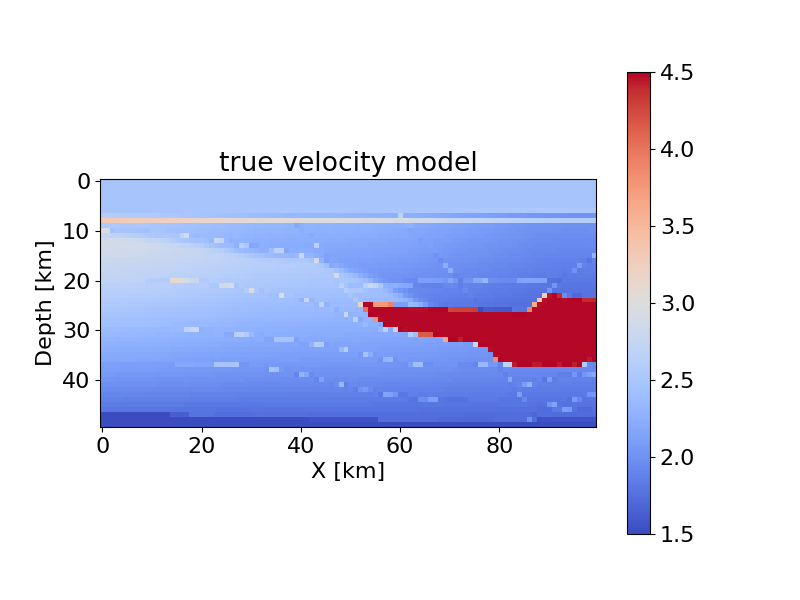
\includegraphics[width=70mm]{public/true}
            \caption*{\raisebox{5mm}{Background truth}}
        \end{minipage} &
        \begin{minipage}[b]{70mm}
            \centering
            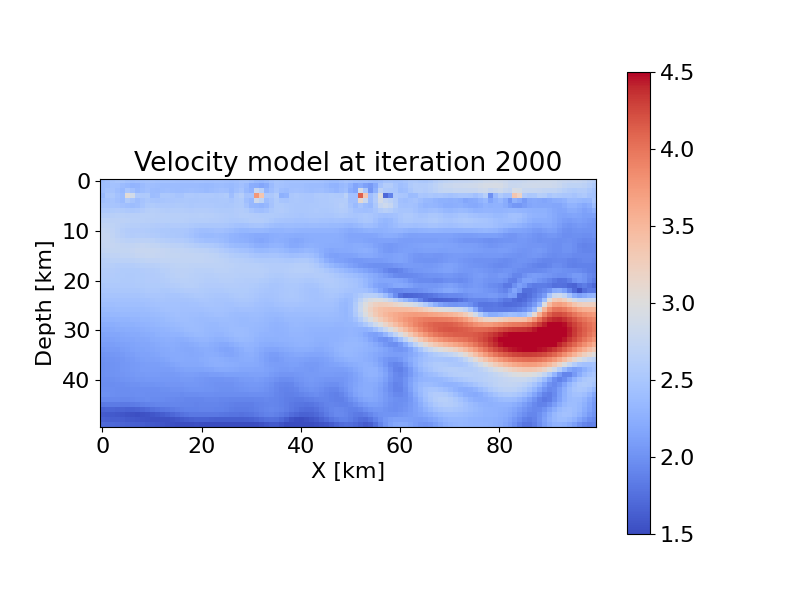
\includegraphics[width=70mm]{public/gradient}
            \caption*{\raisebox{5mm}{Reconstructed with normal FWI}}
        \end{minipage} &
        \multirow[t]{2}{*}{\raisebox{-50mm}{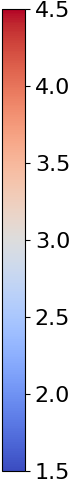
\includegraphics[height=68mm]{public/color-bar}}} \\
        % Second row: Image 3 and 4
        \begin{minipage}[b]{70mm}
            \centering
            
\includegraphics[width=70mm]{public/initial}
            \caption*{Initial model}
        \end{minipage} &
        \begin{minipage}[b]{70mm}
            \centering
            
\includegraphics[width=70mm]{public/pds}
            \caption*{Reconstructed with the constrained FWI}
        \end{minipage} &
    \end{tabular}
    \caption{Velocity models and their corresponding reconstructions.}
    \label{fig:velocity-models}
\end{figure*}

As shown in fig.\ref{fig:velocity-models}, velocity model can be piecewise smooth.
Therefore, We introduce TV constraints to achieve more accurate reconstruction.
Also, by introducing a box constraint, we can ensure that the velocity model does not take invalid values.

We minimize the objective function of the TV and box constrained FWI, which is expressed by the following:
\begin{equation} \label{eq:FWIObjectiveWithTVConstraint} \argmin{\velModel \in \realNumber^N} \ \ \FWIObjectiveWithTVConstraint \end{equation}
where $\alpha \in \realNumber$ is the upper bound of the $l_{1,2}$ norm, and $a, b \in \realNumber$ are the lower and upper bound of the velocity model value, respectively.

The constraints can be integrated into the objective function as indicator functions:
\begin{equation} \label{eq:FWIObjectiveWithTVConstraintWithIndicatorFunction} \argmin{\velModel \in \realNumber^N} \ \ \FWIObjectiveWithTVConstraintWithIndicatorFunction \end{equation}

As mentioned in section~\ref{subsec:mathematical-tools}, $\iota_{\LOneTwoNorm{\cdot} \le \alpha}$ and $\iota_{[a,b]^N}$ can be computed efficiently\eqref{eq:ProximityOperatorForL1Ball}\eqref{eq:ProximityOperatorForL12Ball}.
Therefore, These functions of $E$, $\iota_{[a,b]^N}$ and $\iota_{\LOneTwoNorm{\cdot} \le \alpha}$ correspond to $f$, $g$ and $h$ in \eqref{eq:PDSPrimalEq}, respectively, $\bm{L}$ is corresponds to $\diffOperator$, and the problem~\eqref{eq:FWIObjectiveWithTVConstraintWithIndicatorFunction} can be solved using PDS.
The iterative procedures are as follows:
\begin{equation} \label{eq:FWIWithPDS} \FWIWithPDS \notag \end{equation}

